\section{Single speaker source}\label{ch:single_speaker_source}
This section aims to introduce and analyse the fundamental for a single source, by analyse the behaviour of a baffled circular plane piston source. The pressure around the piston source will be analysed analytically, to determine the radiation of a single speaker from \SI{60}{\hertz} and upwards and compare it with the measurement from \autoref{ch:polar_response}. The \SI{60}{\hertz} lower limit enable the simulation to be validated by measurement in the AAU anechoic chamber and is a used lower limit for the low/mid driver in some line source array \citep{V-DOSC}.  The analyse shall end out with a approximated simulation model of the \gls{dut}.

\subsection{Pressure analysis of a single source}
To characterised the directions properties of an analytical model of the \gls{dut}, the source will be modulated in two dimension as one baffled circular plane piston source. The analysis of a piston source in two dimension built on a thin piston source in three dimension where the x axis is fixed in the plot. This is possible because of vertical beam patten symmetry of \autoref{fig:continues_line_source} \citep{Kinsler2000}. The piston lays flat down so i look like a line source and have radius $a$. The baffled circular plane piston source can be considered as many continuous line sources, which detonate dx and is pointing towards the reader on \autoref{fig:continues_line_source}. The calculated pressure point will be in far field where $r>>a$ holds and the surface integral can be rewritten to a Bessel function \citep{Kinsler2000}. The pressure formula is therefore:

\begin{equation}
p(r,\theta ,t)=\frac{j}{2} \rho_{0}c  \text{\textit{{\LARGE u}}}_{0}\frac{a}{r}ka \left ( \frac{2J_1(ka\, sin(\theta ))}{ka\, sin(\theta )} \right )e^{j(\omega t-kr)}
\end{equation}


Where the complete surface vibrate radially with speed

\begin{equation}
u = \text{\textit{{\LARGE u}}}_{0} \cdot exp(j \omega t)
\end{equation}

    \startexplain
    		\explain{$u$ is the complex speed of the line source }{\si{1}}
        \explain{$\text{\textit{{\LARGE u}}}_{0}$ is the Amplitude}{\si{1}}
        \explain{$j$ is the imaginary unit }{\si{1}}
        \explain{$\omega$ is the angular velocity }{\si{1}}
        \explain{$t$ is the time }{\si{1}}
    \stopexplain
    
Each small sources is treated as an baffled simple source with a width of $dx$ and the source strange can be modulated as following      

\begin{equation}
dQ = \text{\textit{{\LARGE u}}}_{0} 2 a\, sin(\phi) \, dx
\end{equation}

    \startexplain
    		\explain{$dQ$ is the simple source strange }{\si{1}}
        \explain{$\text{\textit{{\LARGE u}}}_{0}$ is the Amplitude}{\si{1}}
        \explain{$a$ is the radius for cylinder }{\si{1}}
        \explain{$\phi$ is the angle between the radius $a$ and the x axis}{\si{1}}
        \explain{$dx$ is the length for the simple source }{\si{1}}
    \stopexplain    
 
The following \autoref{fig:continues_line_source} shows an example of the continues line source where one of the small source is showed with width $dx$ and length $2a \, sin(\phi)$. 

\begin{figure}[H]
	\centering
\begin{picture}(0,0)%
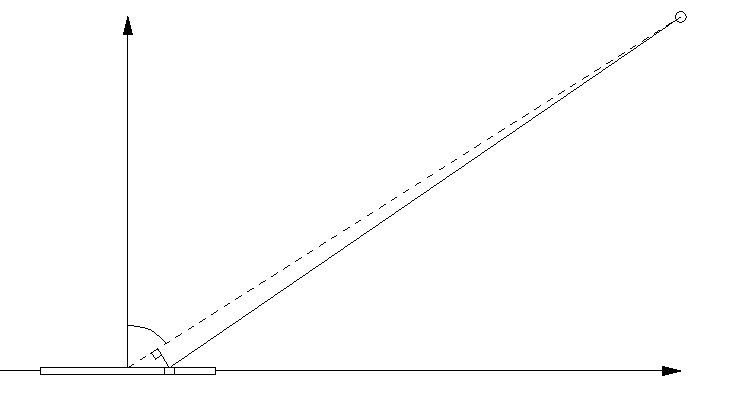
\includegraphics{line_source.pdf}%
\end{picture}%
\setlength{\unitlength}{746sp}%
%
\begingroup\makeatletter\ifx\SetFigFont\undefined%
\gdef\SetFigFont#1#2#3#4#5{%
  \reset@font\fontsize{#1}{#2pt}%
  \fontfamily{#3}\fontseries{#4}\fontshape{#5}%
  \selectfont}%
\fi\endgroup%
\begin{picture}(31223,16833)(-5411,-436)
\put(12106,7139){r'}%
\put(24121,15599){P(r,$\theta$,t)}%
\put(946,2684){$\theta$}%
\put(23851,659){x}%
\put(-89,16094){z}%
\put(11341,8354){r}%
\put(3466,-571){$a$}%
\put(1441,-376){$dx$}%
\put(-134,-421){0}%
\put(-4049,-571){$-a$}%
\put(226,1649){$\Delta$r}%
\end{picture}%
	\caption{The model of a continues line source where y axis is pointing towords the reader. (ref the book)}
		\label{fig:continues_line_source}
\end{figure}




\subsection{Simulation of the \gls{dut} as a piston source and compare to measurement in \autoref{ch:polar_response}}
In this section, the \gls{dut} will be simulated as a baffled circular plane piston source as described in \autoref{ch:single_speaker_source} and compared to the actually measurement of the \gls{dut} \autoref{ax:directional_2}. An piston simulated model of \citep{seas33} in MATLAB shows in \autoref{fig:piston_model_of_seas33}

\begin{figure}[H]
	\centering
	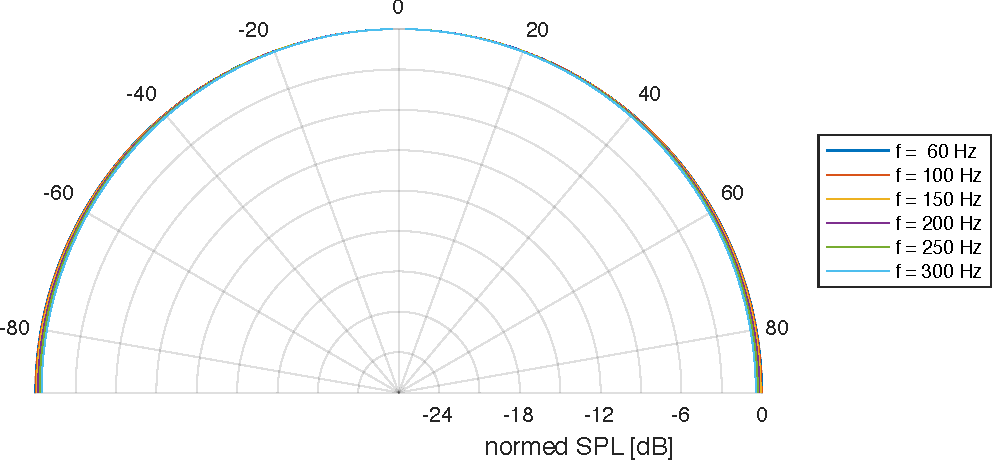
\includegraphics[width=0.8\textwidth]{piston_model.pdf}
	\caption{The figure shows  The \gls{dut} which correspond to this figure is a \citep{seas33}}
		\label{fig:piston_model_of_seas33}
\end{figure}

The actually measurement of the \citep{seas33}  \autoref{ax:directional_2}.

\begin{figure}[H]
	\centering
	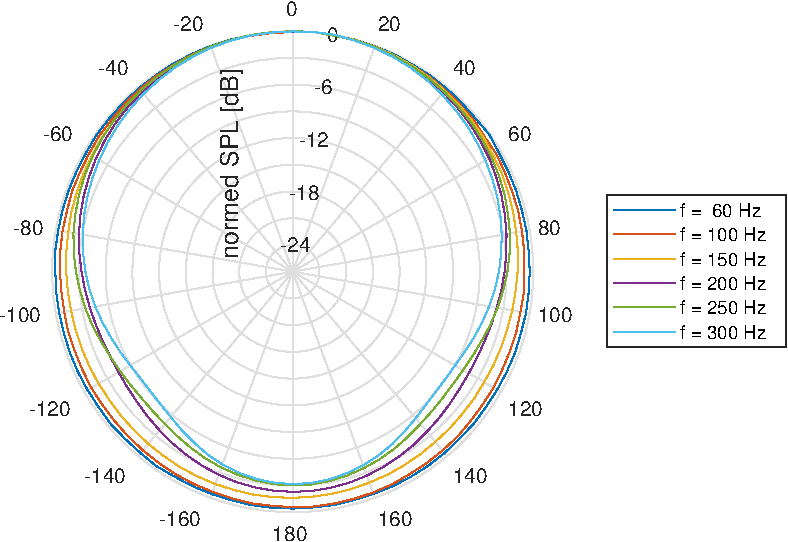
\includegraphics[width=0.8\textwidth]{meas1_seas.pdf}
	\caption{The figure shows  The \gls{dut} which correspond to this figure is a \citep{seas33}}
		\label{fig:speaker_model}
\end{figure}

\subsection{Conclusion}